\documentclass[11pt]{article}

\usepackage{classDM17}
\usepackage{mathtools}
\DeclarePairedDelimiter\ceil{\lceil}{\rceil}
\DeclarePairedDelimiter\floor{\lfloor}{\rfloor}

\title{Asmt 2: Document Similarity and Hashing}
\author{Gopal Menon\\Turn in (\textbf{a pdf}) through Canvas by 2:45pm: \\
Monday, February 13}
\date{}

\begin{document}
\maketitle



\section{Creating k-Grams (40 points)}

\paragraph{A: (20 points)} 
How many distinct $k$-grams are there for each document with each type of $k$-gram? You
should report $4 \times 3 = 12$ different numbers.

    \begin{table}[!h] 
    \centering
    \caption{Number of distinct $k$-grams}
    \begin{tabular}{|c|c|c|c|}
      \hline
   Document  & character $2$-grams &  character $3$-grams & word $2$-grams  \\
      \hline      
      $D1$ &   $330$              &  $1297$  &          $520$                          \\
      \hline      
      $D2$ &    $360$             & $1514$   &           $631$                         \\
      \hline      
      $D3$ &    $353$           &  $1541$  &             $840$                       \\
      \hline      
      $D4$ &      $297$          &  $1023$  &             $412$                       \\
      \hline
    \end{tabular}
    \end{table}

\paragraph{B: (20 points)}  
\paragraph{A: (20 points)}  
Compute the Jaccard similarity between all pairs of documents for each type of $k$-gram.
You should report $3 \times 6 = 18$ different numbers.

\begin{table}[!ht]  
  \centering
  \caption{Jaccard similarity for character $2$-grams}
  \begin{tabular}{|c|c|c|c|c|}
    \cline{2-5}
    \multicolumn{1}{c|}{} & $D1$ & $D2$ & $D3$ & $D4$\\ \hline
    $D1$ &    &    &   & \\ \hline
    $D2$ & $0.8499$   &    &   & \\ \hline
    $D3$ & $0.7740$   & $0.7649$   &   & \\ \hline
    $D4$ & $0.7084$  & $0.7109$  & $0.7241$ & \\ \hline
  \end{tabular}
  \end{table}

\begin{table}[!ht]  
  \centering
  \caption{Jaccard similarity for character $3$-grams}
  \begin{tabular}{|c|c|c|c|c|}
    \cline{2-5}
    \multicolumn{1}{c|}{} & $D1$ & $D2$ & $D3$ & $D4$\\ \hline
    $D1$ &    &    &   & \\ \hline
    $D2$ & $0.6400$   &    &   & \\ \hline
    $D3$ &  $0.4606$  &  $0.4404$  &   & \\ \hline
    $D4$ & $0.3280$  & $0.3125$  & $0.3624$ & \\ \hline
  \end{tabular}
  \end{table}
  
\begin{table}[!ht]  
  \centering
  \caption{Jaccard similarity for word $2$-grams}
  \begin{tabular}{|c|c|c|c|c|}
    \cline{2-5}
    \multicolumn{1}{c|}{} & $D1$ & $D2$ & $D3$ & $D4$\\ \hline
    $D1$ &    &    &   & \\ \hline
    $D2$ &  $0.2579$  &    &   & \\ \hline
    $D3$ &  $0.0334$  & $0.0251$   &   & \\ \hline
    $D4$ &  $0.0054$ &  $0.0058$ & $0.0121$ & \\ \hline
  \end{tabular}
  \end{table}

\section{Min Hashing (30 points)}
\paragraph{A: (25 points)} 
Using grams \textbf{G2}, build a min-hash signature for document $D1$ and $D2$ using $t = \{20, 60, 150, 300, 600\}$ hash functions. For each value of $t$ report the approximate Jaccard similarity between the pair of documents $D1$ and $D2$, estimating the Jaccard similarity:


    \begin{table}[!h] 
    \centering
  \caption{Jaccard similarity between documents $D1$ and $D2$ using character $3$-grams}
    \begin{tabular}{|c|c|c|}
      \hline
   $t$ (number of hash functions)  & Jaccard Similarity  & Error \% \\
      \hline      
      $20$ &   $0.6500$  &   $1.5625$   \\
      \hline      
      $60$ &    $0.6333$  & $1.0469$ \\
      \hline      
      $150$ &    $0.6667$  &  $4.1719$\\
      \hline      
      $300$ &      $0.6800$  &   $6.2500$\\
      \hline
      $600$ &      $0.6817$    & $6.5156$\\
      \hline
      $1200$ &      $0.6625$    & $3.5156$\\
        \hline
      $2400$ &      $0.6571$    & $2.6719$\\
    \hline
    \end{tabular}
    \end{table}
    
\paragraph{B: (5 points)} 
What seems to be a good value for $t$? You may run more experiments. Justify your answer in terms of both accuracy and time.\\

According to the Chernoff-Hoeffding bound, the probability that the average value for the Jaccard Similarity differs from the expected value by a value greater than $\alpha$ after $t$ trials in the case where each value before it is averaged lies between $-\Delta$ and $\Delta$, is given by: 

\begin{equation*}
\begin{aligned}
\Pr \left [ \left |A - \textbf{E} \left (A\right ) \right| > \alpha \right ] \leq 2 \exp \left ( \frac{-t \alpha^2}{2 \Delta^2} \right)
\end{aligned}
\end{equation*}

This means that as we increase the number of hash functions $t$, the probability that the Jaccard Similarity value found by min hashing will differ from the expected value by a large amount will keep falling. However as we increase the number of hash functions, the run time for the computation will increase. \\

From the experiment, it seems that the best value for $t$ is $60$ where the Jaccard Similarity was $0.6333$. However, in another iteration of the experiment, the best value of $0.6338$ was obtained with $2400$ hash functions. 

\section{LSH (30 points)}

\paragraph{A: (8 points)} 

The probability of finding a collision in the hash value for two documents in any of the $r$ bands each containing $b$ hash functions is given by

\begin{equation*}
\begin{aligned}
f(s) = 1 - \left ( 1 - s^b \right ) ^ r
\end{aligned}
\end{equation*}

To find all documents pairs with Jaccard Similarity above $\tau = 0.4$, we should select $b$ and $r$ so that the S-curve has the steepest slope at $s=0.4$. A good estimate for this is given by:

\begin{equation*}
\begin{aligned}
b &\approx -\log_{\tau} \left (k \right )\\
r &= \frac{k}{b}
\end{aligned}
\end{equation*}

where $k$ is the total number of hash functions. Using the values of $k=160$ and $\tau=0.4$, 

\begin{equation*}
\begin{aligned}
b &\approx -\log_{0.4} \left (160 \right )\\
&\approx \floor*{5.5388}\\
&= 5\\
r &= \frac{160}{5}\\
&=32
\end{aligned}
\end{equation*}

Using these values of $r$ and $b$, the S-curve obtained is shown in figure \ref{1stCut}. After some trial and error it was found that with $b=4$ and $r=27$, the S-curve obtained is close to the steepest value at $\tau=0.4$. This is shown in figure \ref{final}.

\begin{figure}[!htb]
\centering
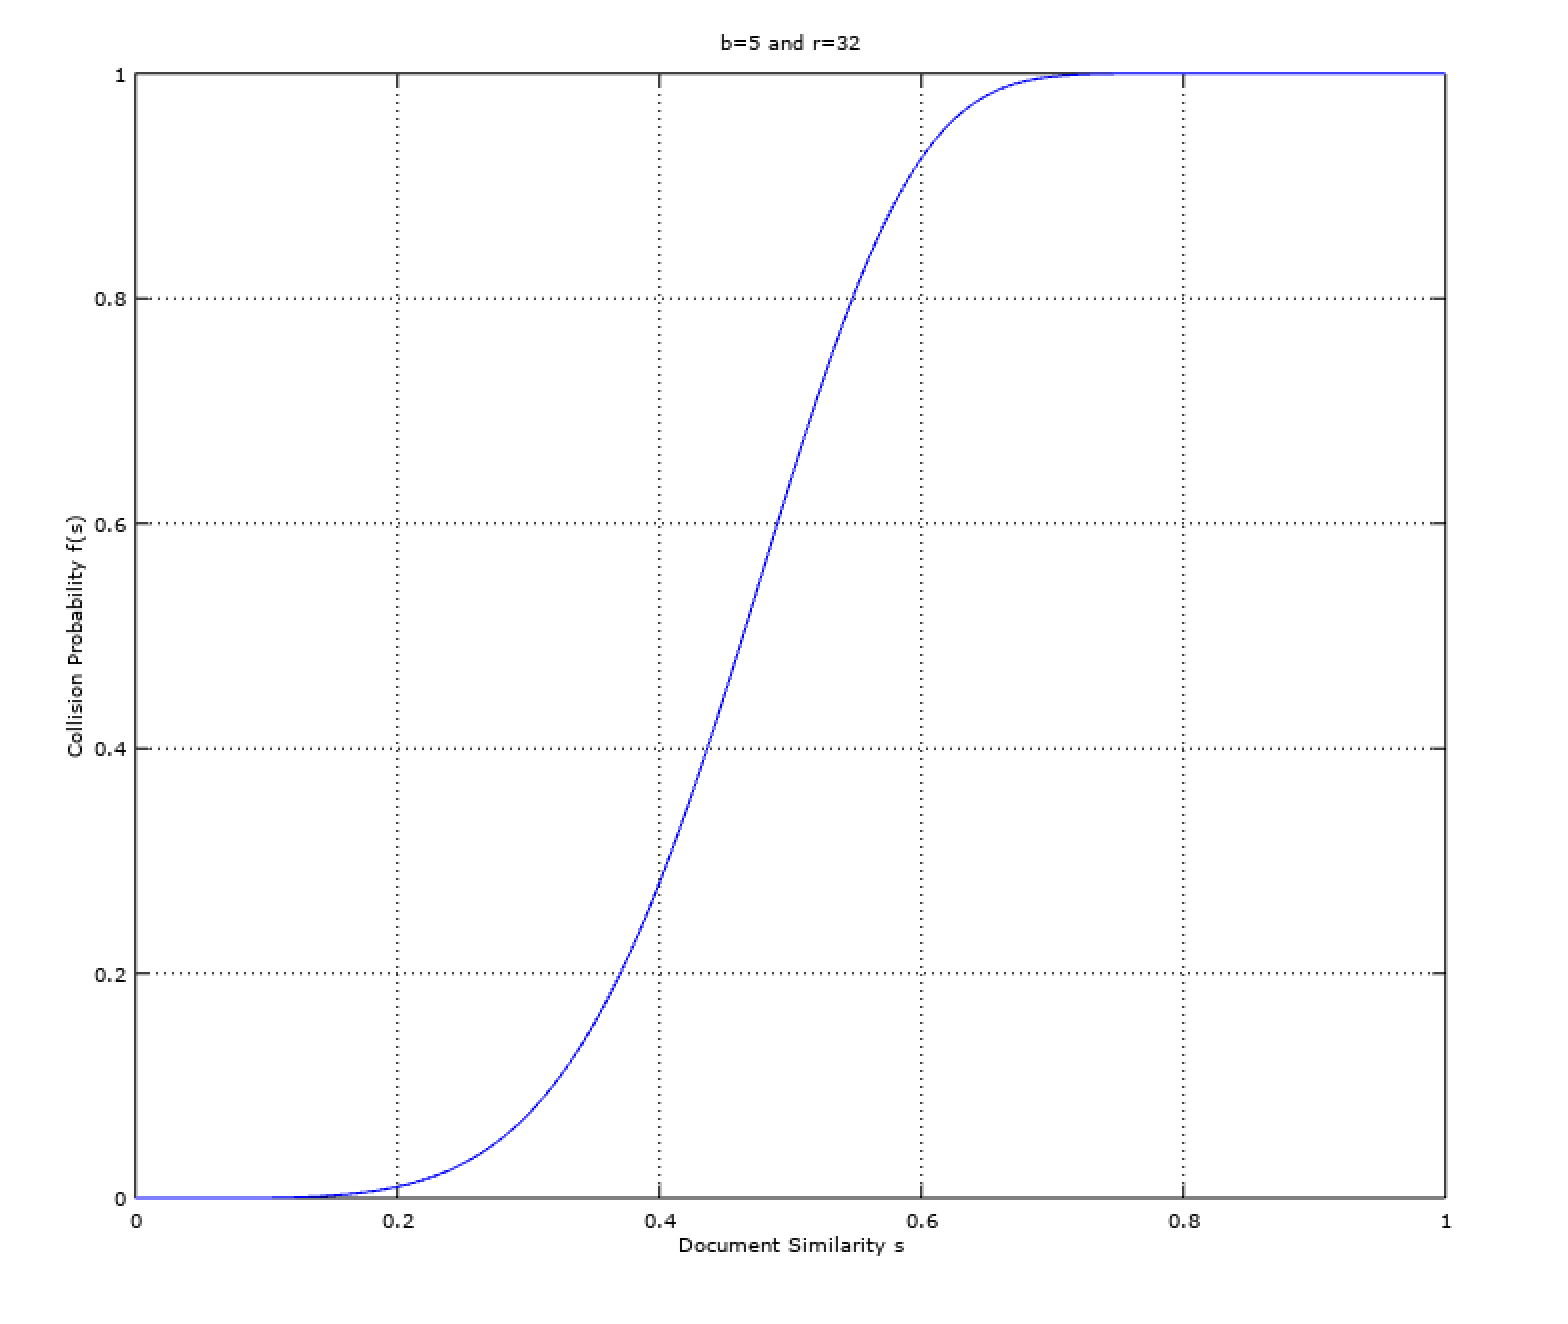
\includegraphics[width=4in]{figures/1stCut.png}
\caption{S-curve with $b=5$ and $r=32$}
\label{1stCut}
\end{figure}

\begin{figure}[!htb]
\centering
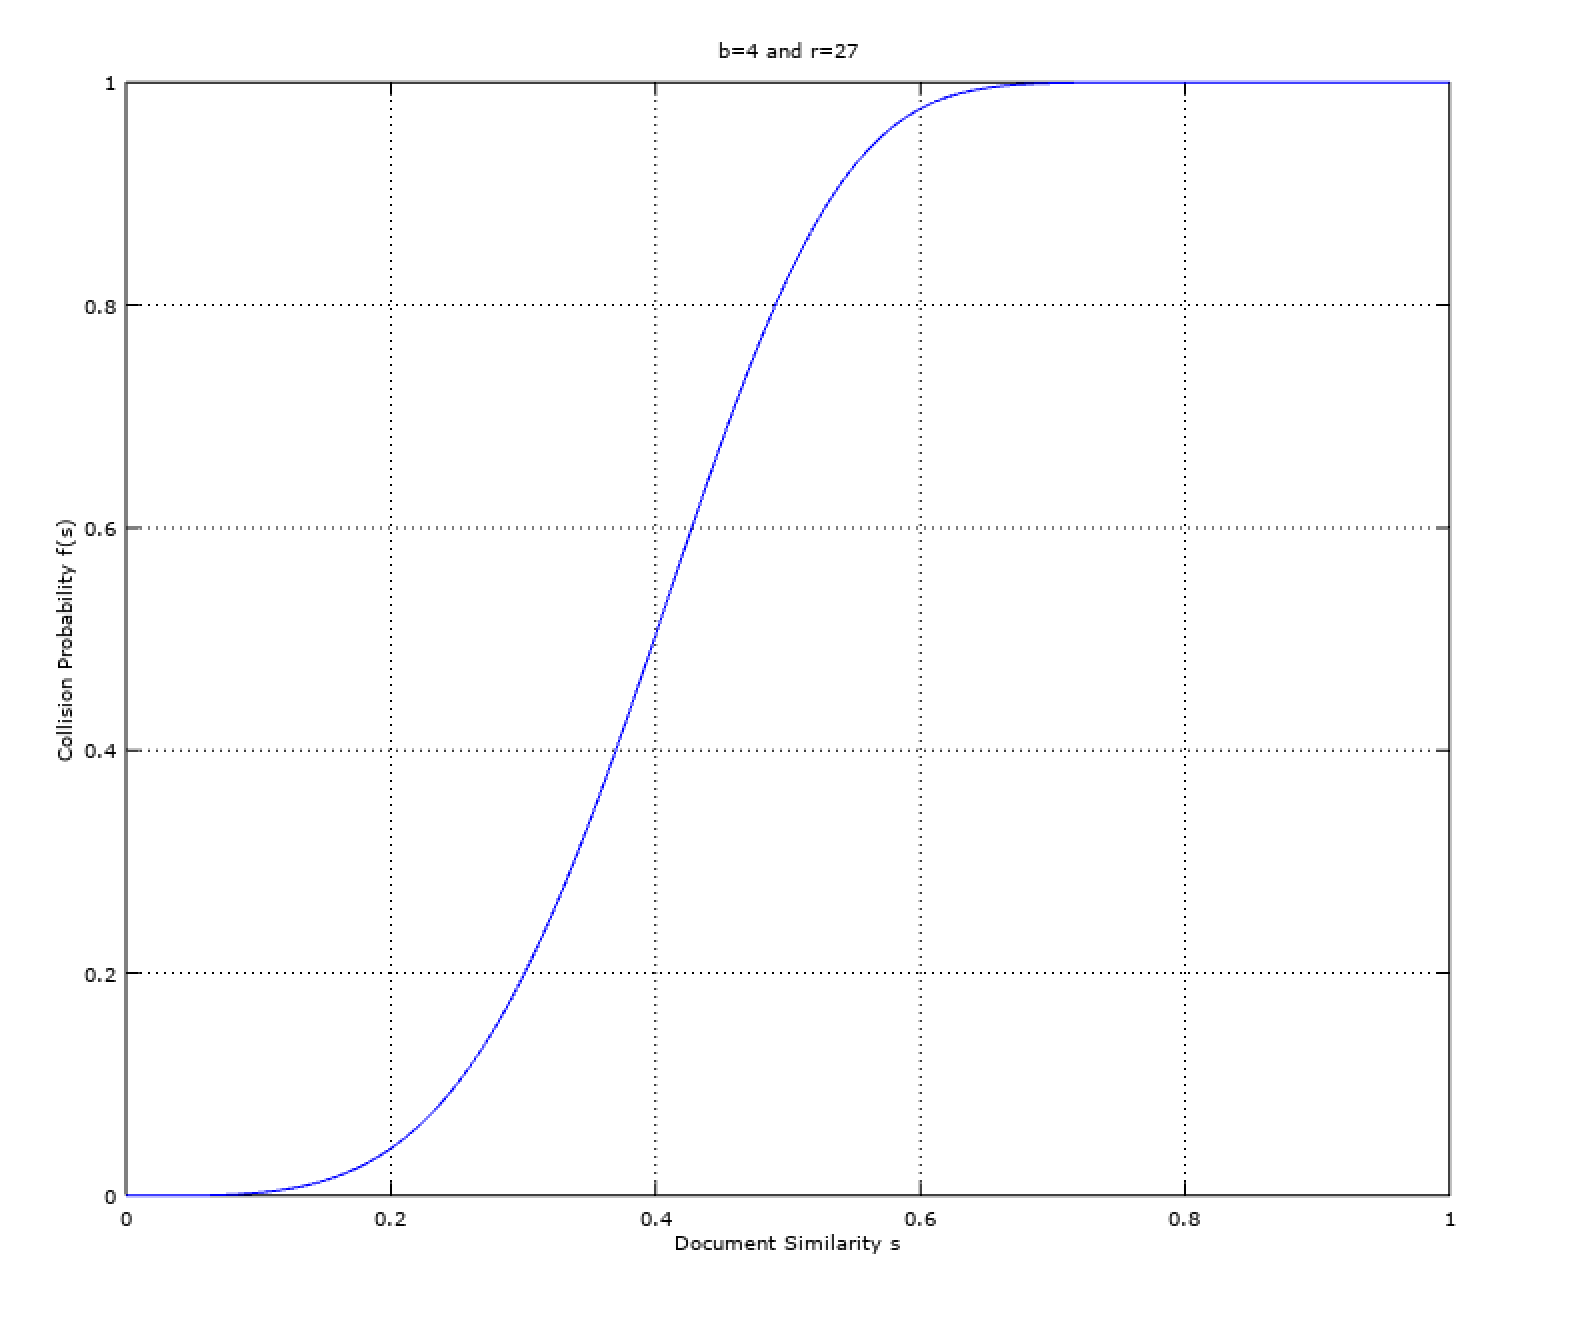
\includegraphics[width=4in]{figures/final.png}
\caption{S-curve with $b=4$ and $r=27$}
\label{final}
\end{figure}

\paragraph{B: (24 points)} 

For the character $3$-grams, the probability of finding the document pairs as being similar as a result of the documents hashing to the same value in at least one of the bands is given below in table \ref{collprob}.

    \begin{table}[!h] 
    \centering
    \caption{Probability of finding a collision}
    \label{collprob}
    \begin{tabular}{|c|c|c|}
      \hline
   Document Pair & Jaccard Similarity $s$ & Collision Probability $f(s) = 1 - \left ( 1 - s^4 \right ) ^ {27}$   \\
      \hline      
      $D1-D2$ &   $0.6400$              &  $0.9930$   \\
      \hline      
      $D1-D3$ &    $0.4606$             & $0.7116$   \\
      \hline      
      $D1-D4$ &    $0.3280$           &  $0.2697$   \\
      \hline      
      $D2-D3$ &      $0.4404$          &  $0.6449$   \\
      \hline
      $D2-D4$ &      $0.3125$          &  $0.2280$   \\
      \hline
      $D3-D4$ &      $0.3624$          &  $0.3749$   \\
      \hline
    \end{tabular}
    \end{table}


\end{document}
